Spočítejte následující plochy:

\begin{enumerate}

	\item  Spočtěte plochu ohraničenou parabolou a přímkou ve výšce $h$ nad vrcholem paraboly.

		\solution{
			Omezující přímka protíná parabolu $y=x^2$ v bodech $(-\sqrt{h},h)$ a $(\sqrt{h},h)$

			hledaná plocha tedy je
			$$2h\sqrt{h} - \int_{-\sqrt{h}}^{\sqrt{h}} x^2 \dx = 2h\sqrt{h} - \left[\frac{x^3}{3}\right]_{-\sqrt{h}}^{\sqrt{h}} = 
			2h\sqrt{h} - \left( \frac{h\sqrt{h}}{3} - \frac{-h\sqrt{h}}{3} \right) = $$
			$$=2h\sqrt{h} - \frac{2h\sqrt{h}}{3} = \frac{4}{3} h\sqrt{h}$$

			Geometrický význam vidíme na Obrázku~\ref{fig:parabola}.
			Hledaná plocha (zobrazena modře) je rozdíl obdélníku ji obsahující (obdélník $[-2, 2] \times [0, 4]$ -- vyplněn modrou nebo zelenou barvou) a integrálu pod parabolou (zobrazen zeleně).
			\begin{figure}[H]
				\centering
				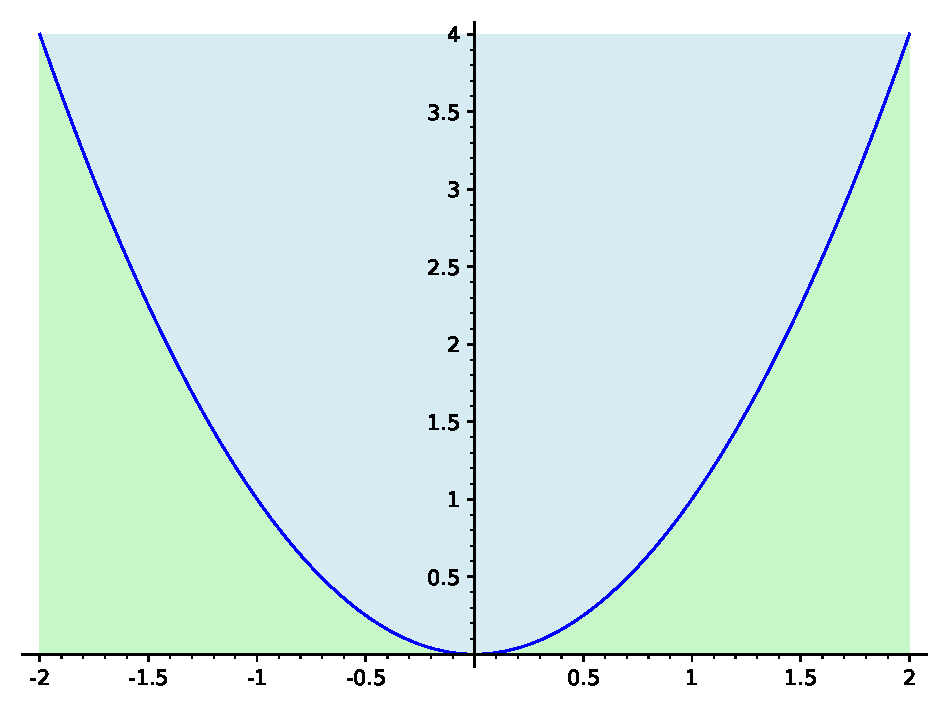
\includegraphics{cviceni_13/fig/parabola.pdf}
				\caption{Plocha mezi parabolou a přímkou ve výšce 4.}
				\label{fig:parabola}
			\end{figure}
		}

	\item  Spočtěte plochu kruhu o poloměru $r$.

		\solution{
			Spočteme plochu čtvrtiny kruhu (a pak vynásobíme čtyřmi), přičemž čtvrtkruh je vlastně ohraničen křivkou $f(x) = \sqrt{r^2-x^2}$

			\begin{align*}
				\int_0^r \sqrt{r^2-x^2} \dx &= \int_0^r \sqrt{r^2(1-\left(\frac{x}{r}\right)^2)} \dx \\
				&= r \int_0^r \sqrt{1-\left(\frac{x}{r}\right)^2} \dx \\
				&\text{zvolíme substituci: } \left( \begin{array}{rcl}  t&=&x/r \\ dt&=&1/r\dx \end{array} \right) \\
				&= r^2 \int_0^1 \sqrt{1-t^2} \dt \\
				&= r^2\left[\frac{1}{2}\left(x\sqrt{1-x^2}+ \arcsin x\right)\right]_0^1 \\
				&= r^2 \left(\frac{1}{2} \cdot \frac{\pi}{2}\right) \\
				&= \frac{\pi r^2}{4} 
			\end{align*}
			
			Z toho dopočteme, že plocha kruhu o poloměru $r$ je $\pi r^2$

			Geometrický význam vidíme na Obrázku~\ref{fig:ctvrtkruh}.
			\begin{figure}[H]
				\centering
				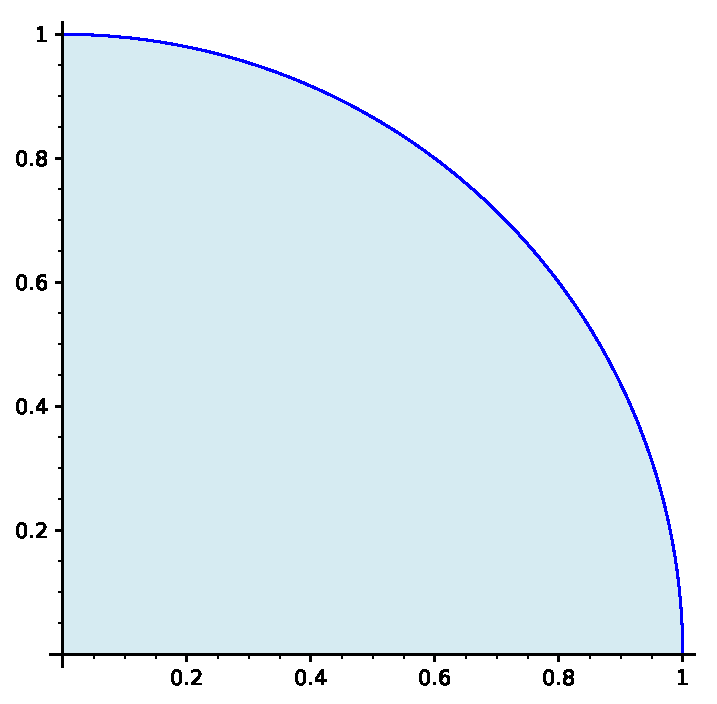
\includegraphics[keepaspectratio]{cviceni_13/fig/ctvrtkruh.pdf}
				\caption{Čtvrtkruh o poloměru 1.}
				\label{fig:ctvrtkruh}
			\end{figure}
		}

	\item  Spočtěte plochu mezi křivkami funkcí $f(x)=x^2-2x+1$ a $g(x)=x^3-x^2-x+1$ (s průsečíky $0$ a $1$).

		\solution{
			$$\int_0^1 g(x) \dx - \int_0^1 f(x) \dx = \int_0^1 (g(x)-f(x)) \dx =$$
			$$= \int_0^1 (x^3-x^2-x+1) - (x^2-2x+1) \dx = \int_0^1 (x^3-2x^2+x) \dx =$$
			$$= \left[\frac{x^4}{4} -2\frac{x^3}{3}+\frac{x^2}{2}\right]_0^1 = 
			\frac{1}{4} - \frac{2}{3} + \frac{1}{2} = \frac{1}{12}$$

			Geometrický význam vidíme na Obrázku~\ref{fig:mezi_polynomy}.
			\begin{figure}[H]
				\centering
				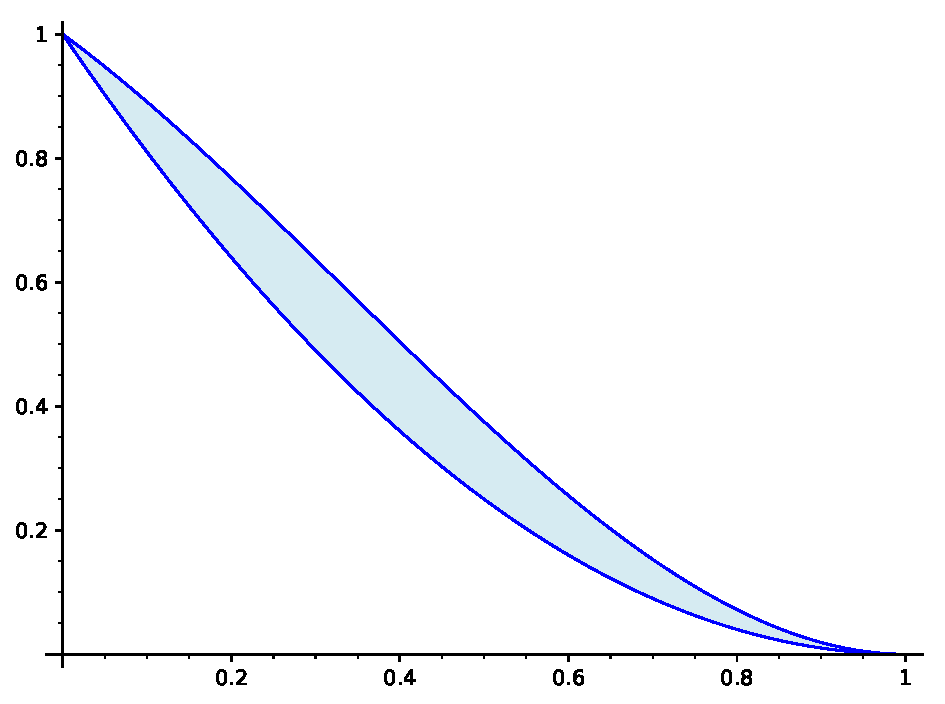
\includegraphics[keepaspectratio]{cviceni_13/fig/mezi_polynomy.pdf}
				\caption{Plocha mezi dvěma polynomy (modře).}
				\label{fig:mezi_polynomy}
			\end{figure}
		}

	\item  Vezměme funkci $\sin x$ na intervalu $(0,\pi)$ a její ``převrácený obraz ukotvený v bodě $(0,1)$'' (funkce $1-\sin x$). 
		Spočtěte plochu útvaru který leží mezi těmito křivkami (taková čočka).

		\solution{
			Průsečíky funkcí jsou body $(a,\frac{1}{2})$, $(\pi-a,\frac{1}{2})$, kde $a = \arcsin(1/2) = \frac{\pi}{6}$

			$$\int_a^{\pi-a} \sin x - (1-\sin x) \dx = \int_a^{\pi-a} (2\sin x - 1) \dx = 
			2\int_a^{\pi-a} \sin x \dx - \int_a^{\pi-a}1 \dx =$$
			$$=2[-\cos x]_a^{\pi-a} - [x]_a^{\pi-a} = -2\cos (\pi-a) +2\cos(a) -((\pi-a)-a) =$$
			$$=2\cos \frac{\pi}{6} - 2\cos\frac{5\pi}{6}- \frac{2\pi}{3} = \frac{2\sqrt{3}}{2} + \frac{2\sqrt{3}}{2} - \frac{2\pi}{3} = 
			2\sqrt{3} - \frac{2\pi}{3} \cong 1.37$$

			Geometrický význam vidíme na Obrázku~\ref{fig:mezi_siny}.
			\begin{figure}[H]
				\centering
				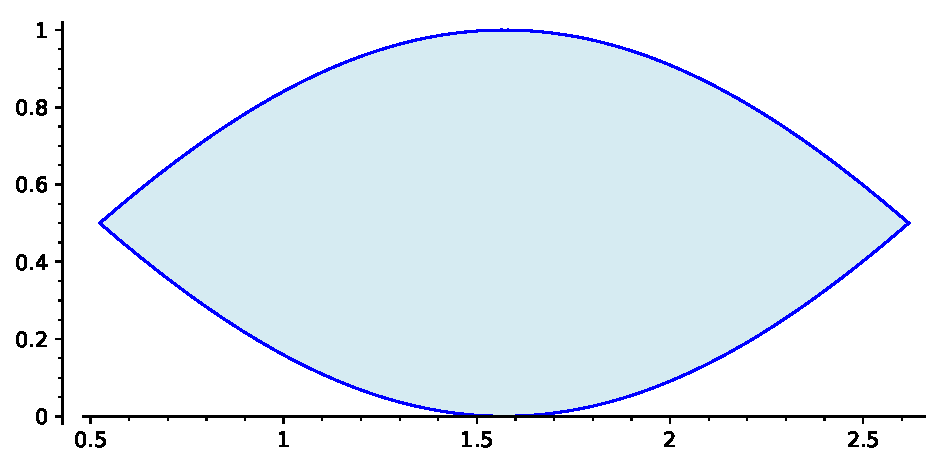
\includegraphics[keepaspectratio]{cviceni_13/fig/mezi_siny.pdf}
				\caption{Čočka mezi dvěma sinusoidami (modře).}
				\label{fig:mezi_siny}
			\end{figure}
		}

\end{enumerate}

